%&goedomteweten
\documentclass[presentatie.tex]{subfiles}

\begin{document}

\section{\texorpdfstring{}{Goed om te weten}}%Goed om te weten}

\clearrecentlist
    
% \begin{frame}{Goed om te weten}
%     TODO Goed om te weten
% \end{frame}

\begin{saveblock}{code}
	\begin{highlightblock}[gobble=8,linewidth=0.5\textwidth,framexleftmargin=0.25em]
        Code
	\end{highlightblock}
\end{saveblock}

\begin{frame}
    {Installatie}

    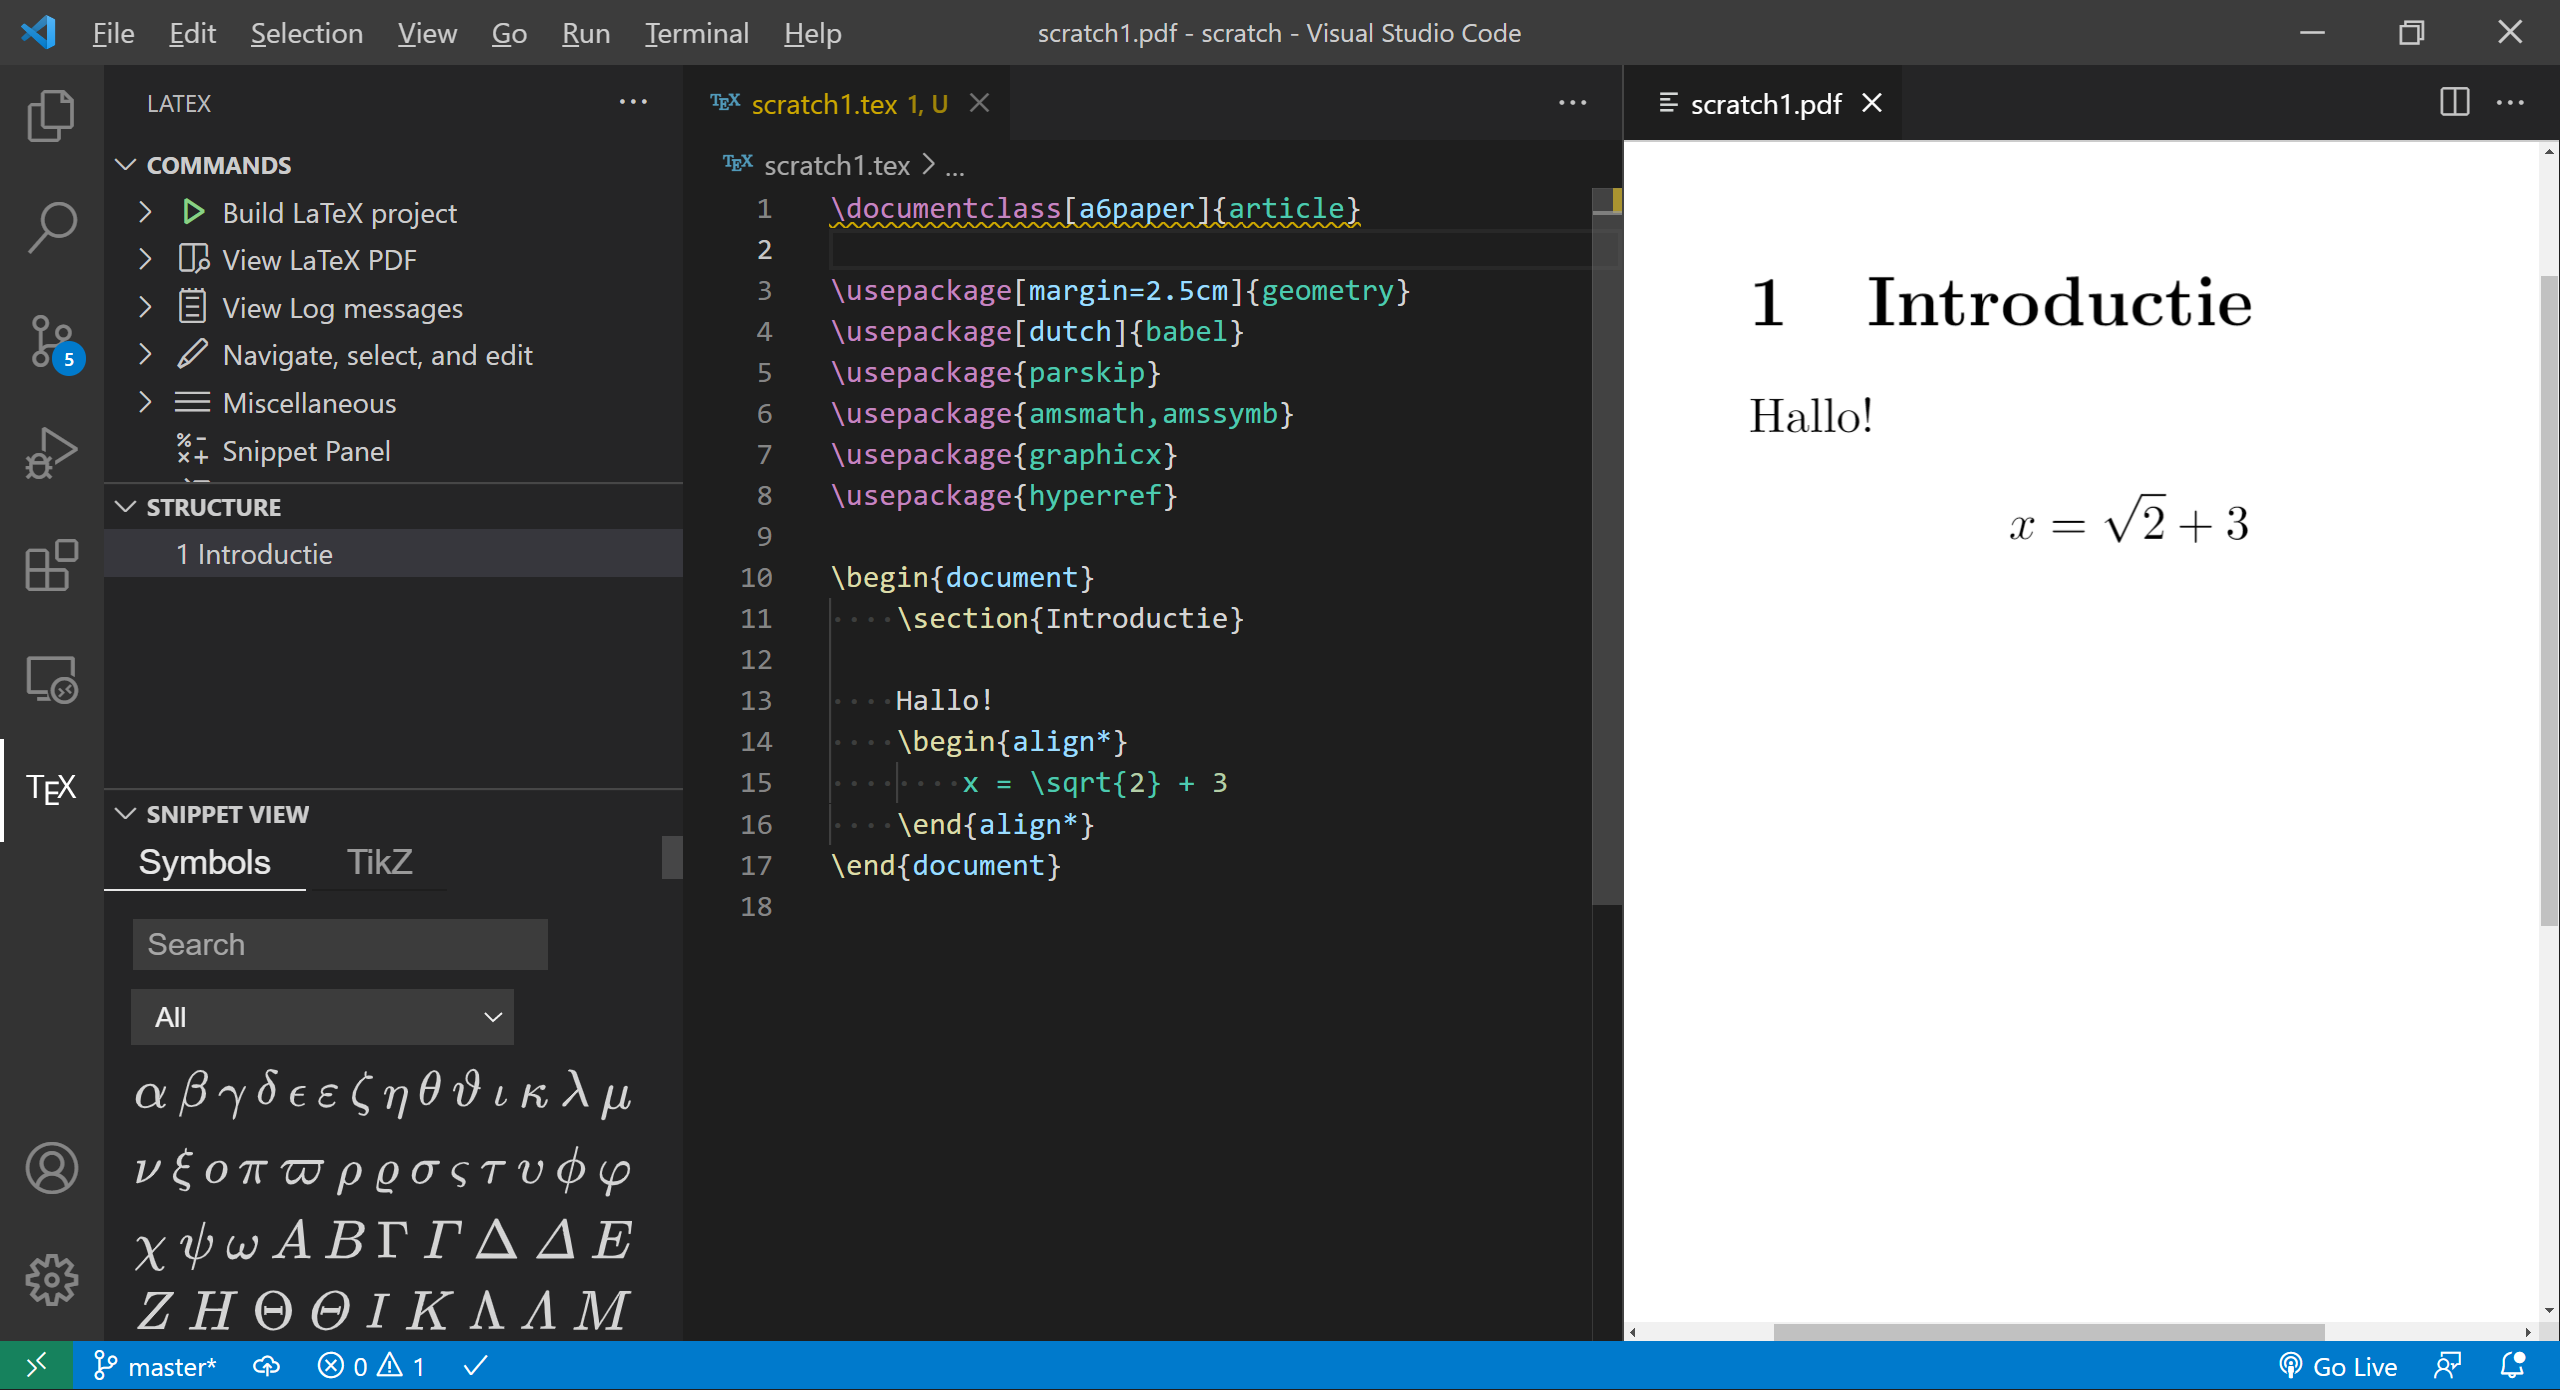
\includegraphics[width=\linewidth,height=0.8\textheight,keepaspectratio]{assets/Misc/VisualStudioCodeDemo.png}
\end{frame}

\begin{frame}
    Op installaties meermaals compileren.
\end{frame}

\begin{frame}{La fin}
	\begin{center}
		\LARGE Vragen?
	\end{center}

    \bigskip
	

    \begin{center}
        Loop je vast? Mail me op\par
        \url{vincent.kuhlmann@hotmail.com}
    \end{center}

    \begin{center}
        De slides en extra materiaal vind je op\par
        \href{https://vkuhlmann.github.io/uavlatex}{\ul{\texttt{vkuhlmann.github.io/uavlatex}}}
    \end{center}
    \begin{center}
        (c) 2021 Vincent Kuhlmann,\par
        Creative Commons CC BY-NC-SA
    \end{center}
\end{frame}

\end{document}
